\newpage
\section{Implementierung}
Dieses Kapitel widmet sich der konkreten Implementierung.

\subsection{\microphone}
Bevor eine Messung mit dem Board durchgeführt worden ist, wurde zuerst ein Plausibilitätscheck vorgenommen. Dabei überprüft man, ob die beiden \microphone \platz Mikrofone korrekte Ergebnisse liefern. Der Aufbau ist durch das folgende Blockschaltbild \ref{img:blockschaltbild_plausibilitaetscheck} abgebildet. Abbildung \ref{img:picture_plausibilitaetscheck} zeigt den Aufbau im Laborraum.

\begin{figure}[H]
\centering
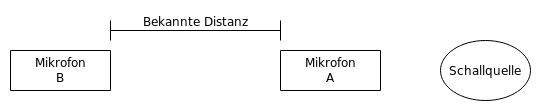
\includegraphics[width=0.9\textwidth]{images/plausibilitaetscheck.png}
\caption{Versuchsaufbau als Blockschaltbild}
\label{img:blockschaltbild_plausibilitaetscheck}
\end{figure}

\begin{figure}[H]
\centering
\hspace*{-1.9cm}
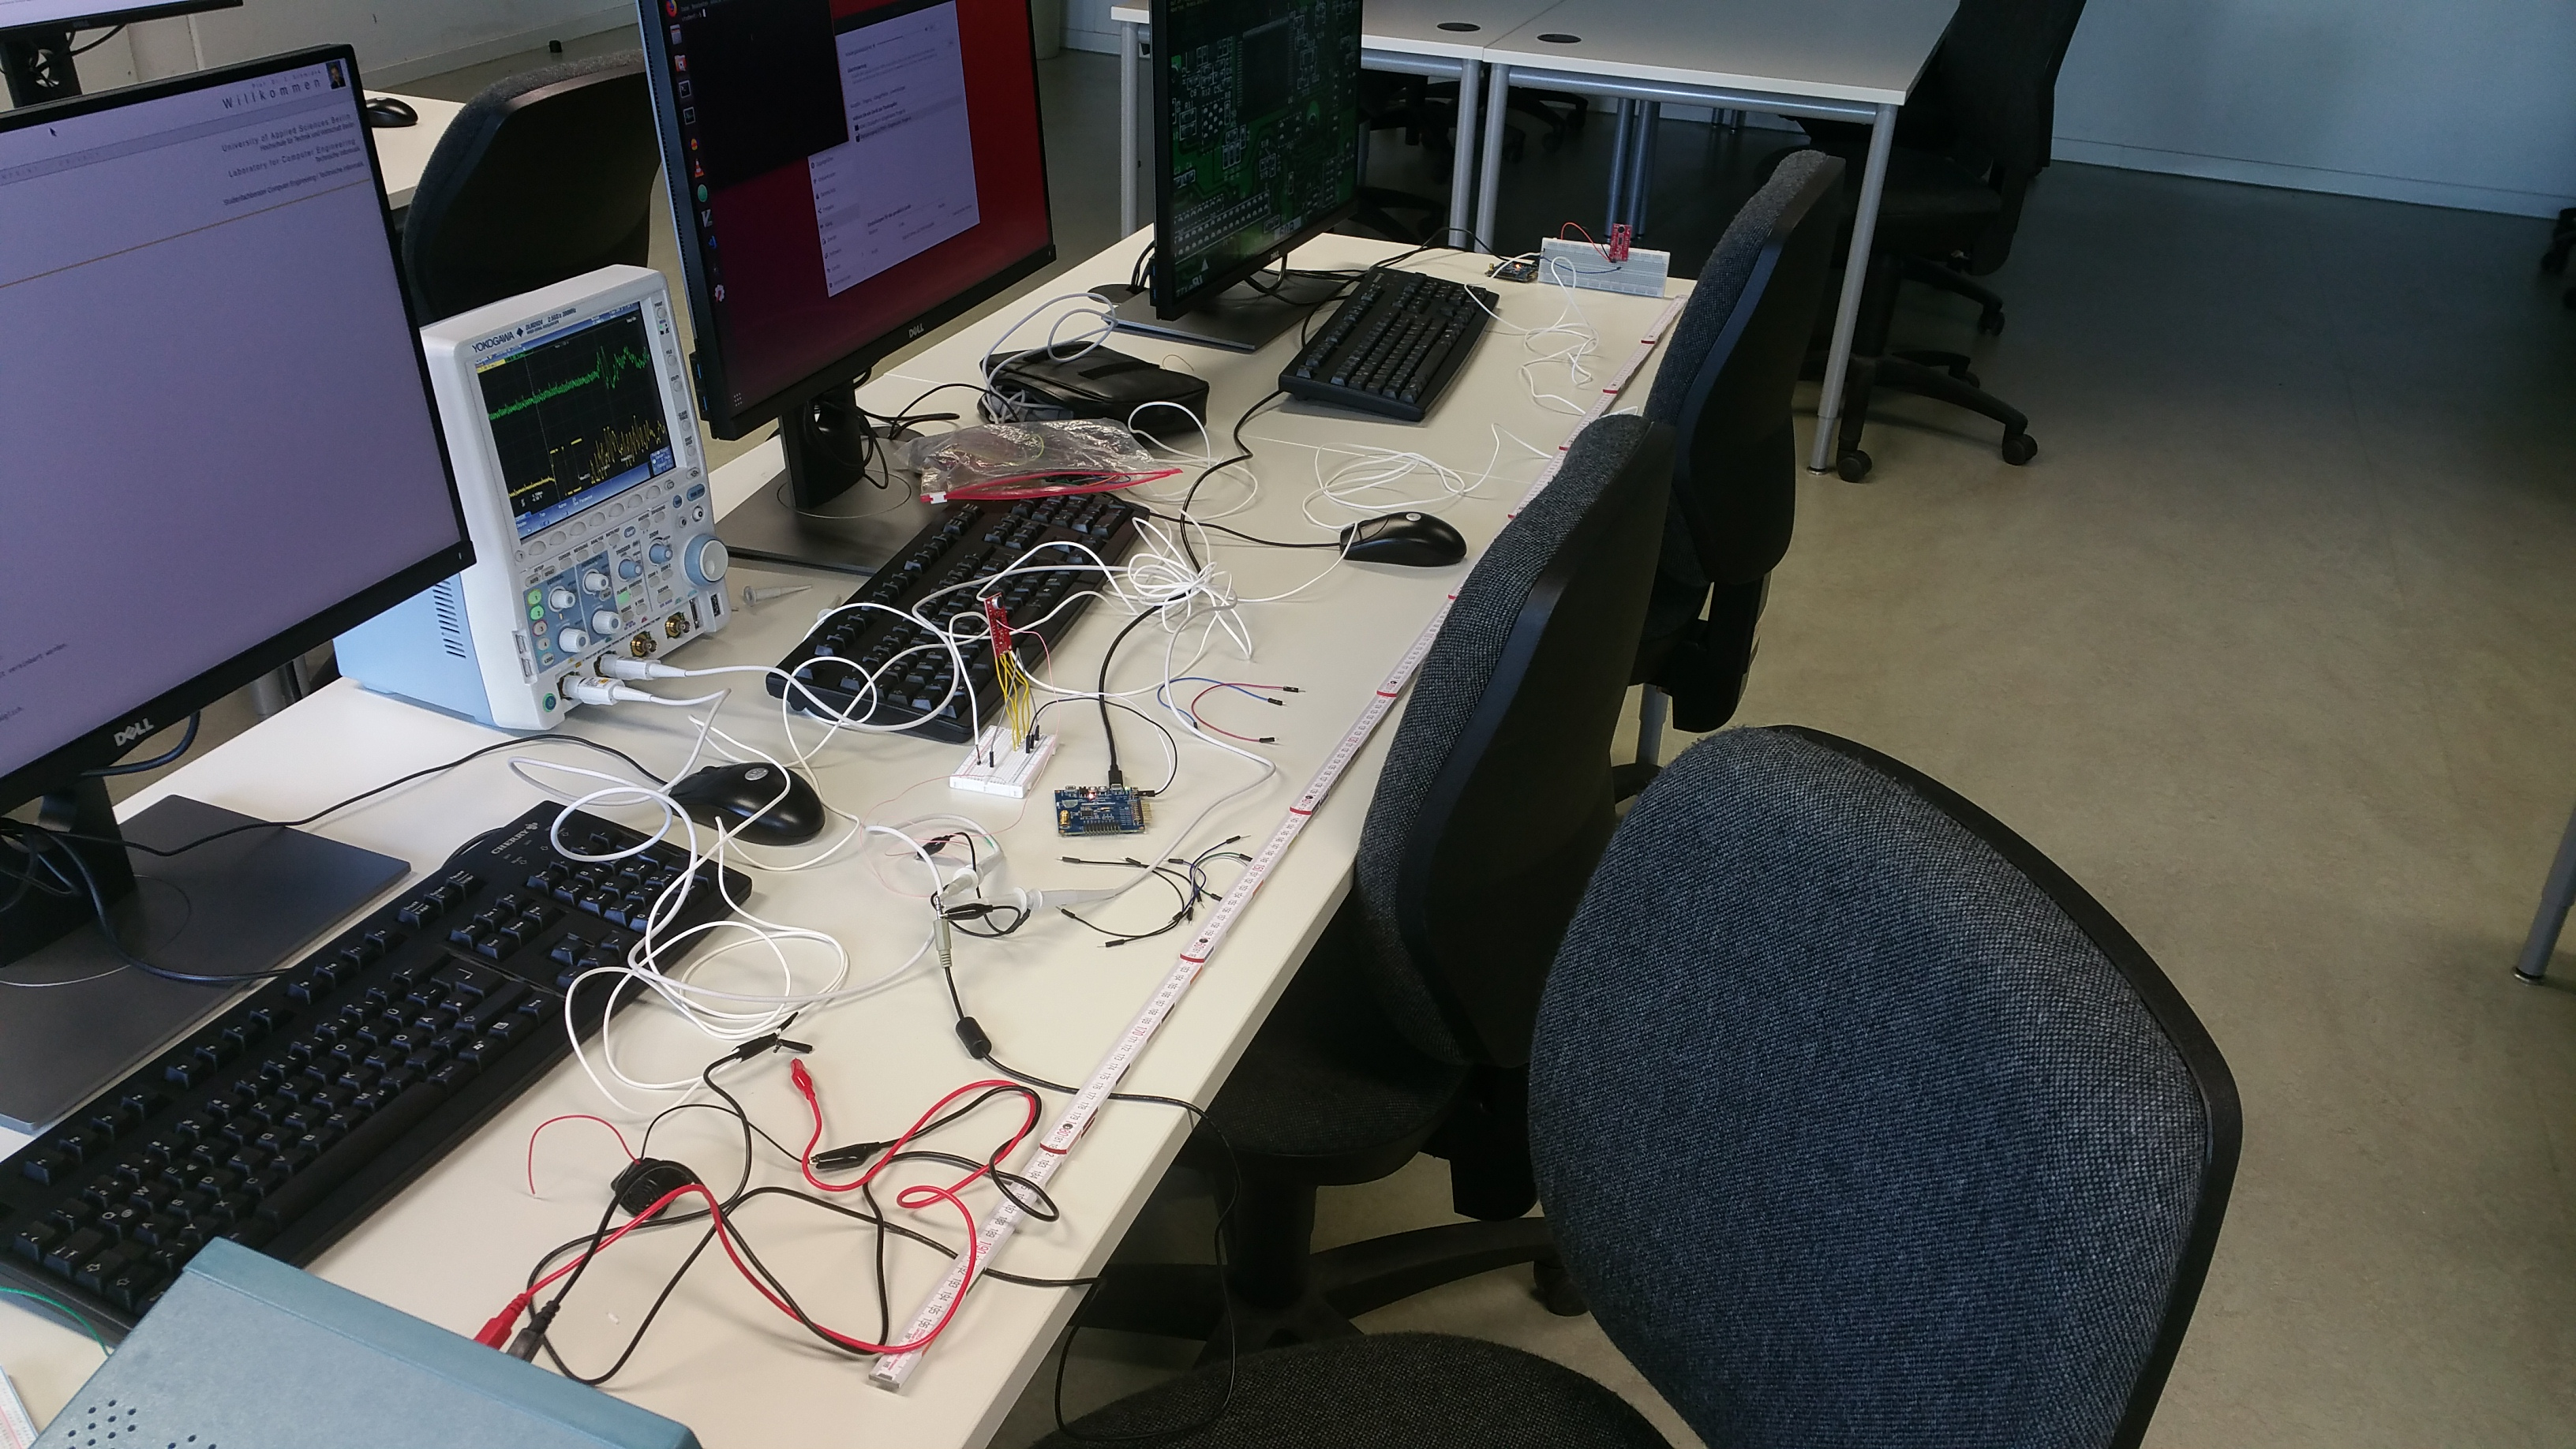
\includegraphics[width=1.2\textwidth]{images/plausibilitaetscheck_sparkfun_foto.jpg}
\caption{Versuchsaufbau}
\label{img:picture_plausibilitaetscheck}
\end{figure}

Die beiden Mikrofone sind an einem Oszilloskop angeschlossen. Es werden die \si{AUDIO}- und \si{GATE}-Ausgänge untersucht. Wenn die Schallquelle einen Ton aussendet (durch Klatschen oder Ähnliches), passiert er zuerst das Mikrofon A und dann mit einer Verzögerung Mikrofon B. Der Abstand der beiden Mikrofone wurde daraufhin mit dem Oszilloskop überprüft. In Abbildung \ref{img:plausibilitaetscheck_oszi} sind vier verschiedene Signale abgebildet. Dabei entspricht Signal \textit{gelb} dem \si{GATE}-Ausgang von Mikrofon A und \textit{grün} dem \si{AUDIO}-Ausgang. Signal \textit{violett} und \textit{blau} entsprechen dem \si{GATE}- und \si{AUDIO}-Ausgang von Mikrofon B. Es ist deutlich erkennbar, dass eine Verzögerung vorhanden ist. Die beiden \si{GATE}-Ausgänge liegen ungefähr \SI{2863}{\micro \second} auseinander. Mit einer Ausbreitungsgeschwindigkeit von \SI{0,034}{\centi\metre\per\micro\second} entspricht das ungefähr \SI{97,342}{\centi\metre}. Der gemessene Abstand beträgt \SI{100}{\centi\metre}. Diese Auswertung zeigt, dass die Verzögerung nur minimal von dem gemessenen Abstand abweicht. Es folgen weitere Messungen, bei dem anstatt eines Klatschens der verwendete Tongeber genommen wird. Dabei sitzt der Lautsprecher direkt neben einem der beiden Mikrofone. Das zweite Mikrofon wird in Abständen von \SI{1}{\metre}, \SI{2}{\metre} und \SI{3}{\metre} aufgestellt. Es folgen drei Tabellen (\ref{tab:plausibilitaetscheck_1m} - \ref{tab:plausibilitaetscheck_3m}) mit den Messwerten (Arithmetisches Mittel).

\begin{figure}[H]
	\centering
	\hspace*{-1.9cm}
	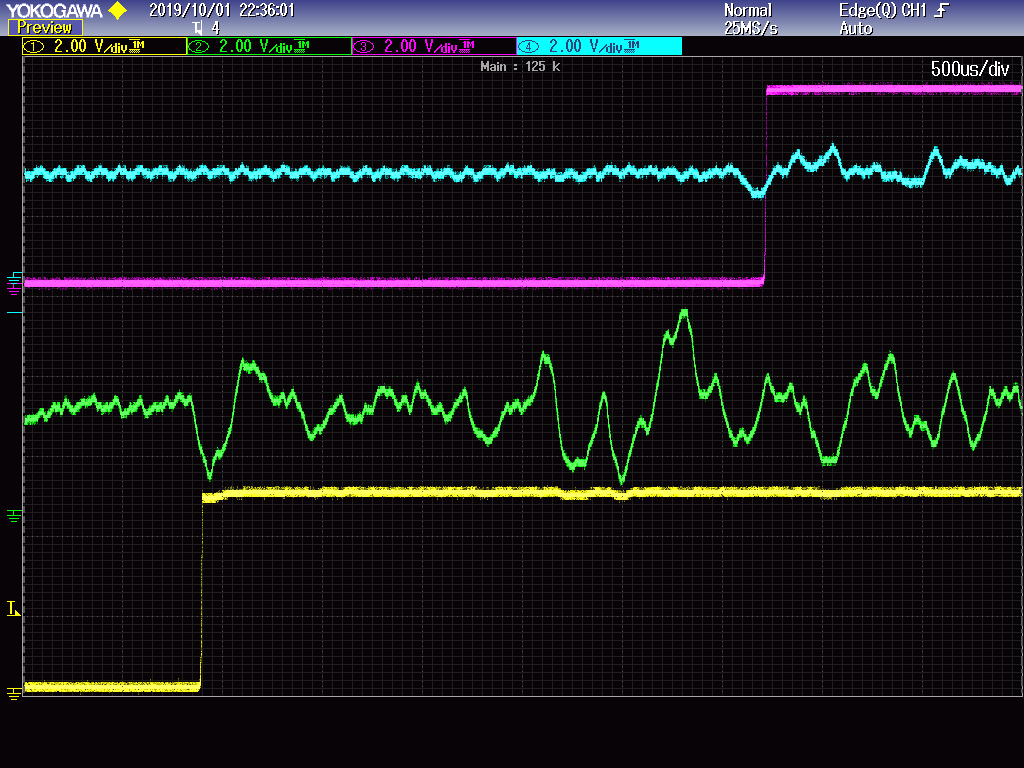
\includegraphics[width=1.2\textwidth]{images/plausibilitaetscheck_oszi.png}
	\caption{Verzögerung der Schallausbreitung}
	\label{img:plausibilitaetscheck_oszi}
\end{figure}

\begin{table}[H]
\centering
\begin{adjustwidth}{-1.4cm}{}
\caption{Messwerte bei \SI{1}{m} Entfernung}
\label{tab:plausibilitaetscheck_1m}
\begin{tabular}{|c|c|c|c|}
\hline
\multicolumn{4}{|c|}{\textbf{\SI{1}{m} Entfernung}}	\\ \hline
\textbf{Messwert von Mikrofon 1 [\si{\mu s}]} & \textbf{Messwert von Mikrofon 2 [\si{\mu s}]} & \textbf{Differenz [\si{\mu s}]} & \textbf{Distanz [\si{\centi\m}]}\\ \hline
\si{595,00}	 & 	\si{4345,00}	 & 	\si{3750,00}	 & 	\si{127,50}	 \\ \hline
\si{603,00}	 & 	\si{4340,00}	 & 	\si{3737,00}	 & 	\si{125,05}	 \\ \hline
\si{461,00}	 & 	\si{4440,00}	 & 	\si{3979,00}	 & 	\si{135,28}	 \\ \hline
\si{608,00}	 & 	\si{4560,00}	 & 	\si{3952,00}	 & 	\si{134,36}	 \\ \hline
\si{641,00}	 & 	\si{4670,00}	 & 	\si{4029,00}	 & 	\si{136,98}	 \\ \hline
\si{443,00}	 & 	\si{4400,00}	 & 	\si{3957,00}	 & 	\si{134,53}	 \\ \hline
\si{450,00}	 & 	\si{4415,00}	 & 	\si{3965,00}	 & 	\si{134,81}	 \\ \hline
\si{634,00}	 & 	\si{4335,00}	 & 	\si{3701,00}	 & 	\si{125,83}	 \\ \hline
\si{638,00}	 & 	\si{4425,00}	 & 	\si{3787,00}	 & 	\si{128,75}	 \\ \hline
\si{640,00}	 & 	\si{4850,00}	 & 	\si{4210,00}	 & 	\si{143,14}	 \\ \hline
\multicolumn{4}{|c|}{\textbf{Durchschnitt}}                    			\\ \hline
\si{571,30}	 & 	\si{4036,50}	 & 	\si{3511,00}	 & 	\si{132,62}	 \\ \hline
\end{tabular}
\end{adjustwidth}
\end{table}


\begin{table}[H]
\centering
\begin{adjustwidth}{-1.4cm}{}
\caption{Messwerte bei \SI{2}{m} Entfernung}
\label{tab:plausibilitaetscheck_2m}
\begin{tabular}{|c|c|c|c|}
\hline
\multicolumn{4}{|c|}{\textbf{\SI{2}{m} Entfernung}} \\ \hline
\textbf{Messwert von Mikrofon 1 [\si{\mu s}]} & \textbf{Messwert von Mikrofon 2 [\si{\mu s}]} & \textbf{Differenz [\si{\mu s}]} & \textbf{Distanz [\si{\centi\m}]}\\ \hline
\si{476,00}	 & 	\si{20150,00}	 & 	\si{19674,00}	 & 	\si{668,91}	 \\ \hline
\si{458,00}	 & 	\si{37900,00}	 & 	\si{37442,00}	 & 	\si{1273,02}	 \\ \hline
\si{471,00}	 & 	\si{36150,00}	 & 	\si{35679,00}	 & 	\si{1213,08}	 \\ \hline
\si{681,00}	 & 	\si{38750,00}	 & 	\si{38079,00}	 & 	\si{1294,68}	 \\ \hline
\si{452,00}	 & 	\si{38150,00}	 & 	\si{37698,00}	 & 	\si{1281,73}	 \\ \hline
\si{466,00}	 & 	\si{34150,00}	 & 	\si{33684,00}	 & 	\si{1145,25}	 \\ \hline
\si{675,00}	 & 	\si{38750,00}	 & 	\si{38075,00}	 & 	\si{1294,55}	 \\ \hline
\si{450,00}	 & 	\si{33550,00}	 & 	\si{33100,00}	 & 	\si{1125,40}	 \\ \hline
\si{447,00}	 & 	\si{32600,00}	 & 	\si{32153,00}	 & 	\si{1093,20}	 \\ \hline
\si{460,00}	 & 	\si{35800,00}	 & 	\si{35340,00}	 & 	\si{1201,56}	 \\ \hline
\multicolumn{4}{|c|}{\textbf{Durchschnitt}}                   	 		\\ \hline
\si{503,60}	 & 	\si{34595,00}	 & 	\si{34072,40}	 & 	\si{1159,13}	 \\ \hline
\end{tabular}
\end{adjustwidth}
\end{table}

\begin{table}[H]
\centering
\begin{adjustwidth}{-1.4cm}{}
\caption{Messwerte bei \SI{3}{m} Entfernung}
\label{tab:plausibilitaetscheck_3m}
\begin{tabular}{|c|c|c|c|}
\hline
\multicolumn{4}{|c|}{\textbf{\SI{3}{m} Entfernung}} \\ \hline
\textbf{Messwert von Mikrofon 1 [\si{\mu s}]} & \textbf{Messwert von Mikrofon 2 [\si{\mu s}]} & \textbf{Differenz [\si{\mu s}]} & \textbf{Distanz [\si{\centi\m}]}\\ \hline
\si{454,00}	 & 	\si{33450,00}	 & 	\si{32996,00}	 & 	\si{1121,86}	 \\ \hline
\si{428,50}	 & 	\si{35800,00}	 & 	\si{35371,50}	 & 	\si{1202,63}	 \\ \hline
\si{474,00}	 & 	\si{37650,00}	 & 	\si{37176,00}	 & 	\si{1263,98}	 \\ \hline
\si{429,00}	 & 	\si{33500,00}	 & 	\si{33071,00}	 & 	\si{1124,41}	 \\ \hline
\si{437,50}	 & 	\si{37700,00}	 & 	\si{37262,50}	 & 	\si{1266,92}	 \\ \hline
\si{439,50}	 & 	\si{35550,00}	 & 	\si{35110,50}	 & 	\si{1193,75}	 \\ \hline
\si{435,50}	 & 	\si{25200,00}	 & 	\si{24764,50}	 & 	\si{841,99}	 \\ \hline
\si{437,50}	 & 	\si{23800,00}	 & 	\si{23362,50}	 & 	\si{794,32}	 \\ \hline
\si{430,00}	 & 	\si{24950,00}	 & 	\si{24520,00}	 & 	\si{833,68}	 \\ \hline
\si{427,50}	 & 	\si{25800,00}	 & 	\si{25372,50}	 & 	\si{862,66}	 \\ \hline
\multicolumn{4}{|c|}{\textbf{Durchschnitt}}                 			\\ \hline
\si{439,30}	 & 	\si{31340,00}	 & 	\si{30900,70}	 & 	\si{1050,62}	 \\ \hline
\end{tabular}
\end{adjustwidth}
\end{table}

Aus den obigen Tabellen ist zu erkennen, dass Mikrofon \si{1} mindestens \SI{439,30}{\mu\s} benötigt, um den Ton wahrzunehmen. Allerdings steht das Mikrofon \si{1} direkt neben dem Tongeber. Durch Latenzen beim Mikrofon ist dieser Messwert nicht null. Allerdings nimmt die Latenz mit der Entfernung ab, woraus keine konstante Abweichung entnommen werden kann. Weiterhin ist zu erkennen, dass es eine deutliche Abweichung gibt, obwohl der Versuch mit Klatschen als Tongeber ein brauchbares Ergebnis produzierte. Dieses Messergebnis zeigt, dass der Lautsprecher und das Mikrofon zusammen keine brauchbaren Messergebnisse erzielen, da die Abweichungen irregulär ansteigen.

\subsection{Modul A}
Das Modul A untersucht die Verzögerung des Masters vom Detektieren eines Mikrofons zu dem Aufruf der Interruptroutine. Das Mikrofon liefert bei Erkennen eines Tons einen Pegelwechsel von \si{LOW} - \si{HIGH}. In der Interruptroutine des Masters wird ein Pin auf \si{HIGH} gesetzt. Dabei besitzt der Slave den Lautsprecher. Es wird ein \si{PIEP}-Ton erzeugt. Master und Slave agieren unabhängig voneinander. Das Oszilloskop wurde an dem \si{GATE}-Ausgang des Mikrofons sowie an dem Pin angehängt, der in der Interruptroutine auf \si{HIGH} gesetzt worden ist. Darüber hinaus ist die Schallquelle dreimal versetzt worden, um Abweichungen abhängig von der Distanz vornehmen zu können. Es folgt eine Tabelle (\ref{tab:modul_A}) mit den Messwerten. Die Messwerte wurden von dem Oszilloskop abgelesen.

\begin{table}[H]
\centering
\caption{ISR-Verzögerung Mikrofon-\board \platz bei unterschiedlicher Kabellänge}
\label{tab:modul_A}
\begin{tabular}{|c|c|c|}
\hline
\multicolumn{3}{|c|}{\textbf{Messwert [\si{\mu s}]}} \\ \hline
\textbf{\SI{1}{\m}}   & \textbf{\SI{2}{\m}}   & \textbf{\SI{3}{\m}}   \\ \hline
\si{67,00}	 & 	\si{91,00}	 & 	\si{66,00}	 \\ \hline
\si{78,00}	 & 	\si{83,00}	 & 	\si{88,50}	 \\ \hline
\si{94,00}	 & 	\si{86,00}	 & 	\si{72,50}	 \\ \hline
\si{81,50}	 & 	\si{59,00}	 & 	\si{75,50}	 \\ \hline
\si{78,50}	 & 	\si{82,00}	 & 	\si{83,00}	 \\ \hline
\si{87,50}	 & 	\si{76,00}	 & 	\si{82,50}	 \\ \hline
\si{74,00}	 & 	\si{87,50}	 & 	\si{92,50}	 \\ \hline
\si{87,00}	 & 	\si{80,00}	 & 	\si{84,50}	 \\ \hline
\si{88,50}	 & 	\si{88,00}	 & 	\si{88,00}	 \\ \hline
\si{81,50}	 & 	\si{70,50}	 & 	\si{64,50}	 \\ \hline
\multicolumn{3}{|c|}{\textbf{Durchschnitt}}      \\ \hline
\si{74,45}	 & 	\si{81,30}	 & 	\si{79,75}	 \\ \hline
\end{tabular}
\end{table}

Die resultierenden Durchschnittswerte (arithmetisches Mittel) weichen nur minimal voneinander ab. Somit hat die Distanz zwischen der Schallquelle und dem Mikrofon keinen Einfluss auf die Interruptzeit. Da die Interruptzeit nur minimal abweicht, kann diese Verzögerung vernachlässigt werden.

\subsection{Modul B}
Dieses Modul untersucht die Abweichungen vom Aussenden eines \si{HIGH}-Signals des Masters bis zum Durchschalten des Mosfets beim Slave. Der Slave nimmt das \si{HIGH}-Signal vom Master durch eine Interruptroutine entgegen und setzt den \si{GATE}-Pin des Mosfets sofort auf \si{HIGH}. Der Master ist per Kabel mit dem Slave verbunden. Für dieses Modul wird kein Lautsprecher und kein Mikrofon benötigt.
\\
Es wird angenommen, dass die Interruptzeit nicht von der Kabellänge zwischen Master und Slave abhängig ist. Die Messwerte für eine Kabellänge von \SI{5}{\m} und einer direkten Verbindung sind wie folgt:

\begin{table}[H]
\centering
\caption{Verzögerung der Slave-ISR bei unterschiedlicher Kabellänge}
\label{tab:modul_B}
\begin{tabular}{|c|l|}
\hline
\multicolumn{2}{|c|}{\textbf{Messwert [\si{\mu s}]}}     \\ \hline
\textbf{Direkte Verbindung}  & \textbf{\SI{5}{\m}} \\ \hline
\si{78,10}	 & 	\si{92,00}	 \\ \hline
\si{70,80}	 & 	\si{74,00}	 \\ \hline
\si{68,30}	 & 	\si{87,00}	 \\ \hline
\si{78,10}	 & 	\si{91,80}	 \\ \hline
\si{74,70}	 & 	\si{84,80}	 \\ \hline
\si{97,20}	 & 	\si{89,60}	 \\ \hline
\si{81,20}	 & 	\si{70,40}	 \\ \hline
\si{94,60}	 & 	\si{90,80}	 \\ \hline
\si{94,50}	 & 	\si{76,80}	 \\ \hline
\si{88,80}	 & 	\si{67,40}	 \\ \hline
\multicolumn{2}{|c|}{\textbf{Durchschnitt}} \\ \hline
\si{82,46}	 & 	\si{82,63}	 \\ \hline
\end{tabular}
\end{table}

Hier zeigt sich, das die Interruptzeit nicht von der Kabellänge abhängig ist. Weiterhin ist die Interruptzeit des Slaves nahezu konstant -- dadurch kann auch diese Verzögerung weg gerechnet werden.

\subsection{Modul C}
Das Modul C soll die Anstiegszeit des N-Mosfets ermitteln. Die Anstiegszeit liegt laut Datenblatt bei \SI{40}{\nano\s}. Das verwendete Oszilloskop schafft es nicht, die Angabe zu überprüfen, da die Zeitauflösung nicht genau genug ist. Die Anstiegszeit verursacht eine Abweichung von $\si{0,000034}[\si{\centi\m\per\nano\s}] \cdot \si{40} [\si{\nano\s}] = \si{0,00136} [\si{\centi\m}]$. Diese Abweichung ist zu gering, um Einfluss auf das Endergebnis auszuüben, da sie erst ab der dritten Nachkommastelle Einfluss ausübt. Aufgrund dessen wird diese Abweichung vernachlässigt.

\subsection{Modul D}
\label{sec:modul_D}
Dieses Modul untersucht die Abweichungen vom Lautsprecher und dem Mikrofon. Dabei wird die Zeit zwischen dem Lautsprecher und dem \si{GATE}-Signal des \microphone s \platz gemessen. Der Master-knoten wird nicht benötigt. Der Slaveknoten besitzt den Lautsprecher und den dazugehörigen Mosfet. Er schaltet den Lautsprecher für \SI{40000}{\mu\s} an. Theoretisch muss der errechnete Wert aus der Distanz und der Schallgeschwindigkeit den gemessenen Werten auf dem Oszilloskop entsprechen. Messungen werden mit den Distanzen \SI{1}{m}, \SI{2}{m} und \SI{3}{m} vorgenommen. Es folgen drei Tabellen (\ref{tab:modul_D_1} - \ref{tab:modul_D_3}) mit den Messwerten.

\begin{table}[H]
\centering
\caption{Abweichung zwischen Mikrofon und Lautsprecher bei \SI{1}{m}}
\label{tab:modul_D_1}
\begin{tabular}{|c|c|c|c|}
\hline
\multicolumn{4}{|c|}{\textbf{\SI{1}{\m} Entfernung}} \\ \hline
\textbf{Theorie [\si{ms}]} & \textbf{Messwert [\si{ms}]} & \multicolumn{1}{l|}{\textbf{Differenz [\si{ms}]}} & \multicolumn{1}{l|}{\textbf{Distanz [\si{cm}]}} \\ \hline
\si{2,94} & \si{5,14} & \si{2,19} & \si{74,76} \\ \hline
\si{2,94} & \si{5,14} & \si{2,19} & \si{74,76} \\ \hline
\si{2,94} & \si{4,87} & \si{1,92} & \si{65,58} \\ \hline
\si{2,94} & \si{4,87} & \si{1,92} & \si{65,58} \\ \hline
\si{2,94} & \si{5,15} & \si{2,20} & \si{75,10} \\ \hline
\si{2,94} & \si{4,88} & \si{1,93} & \si{65,92} \\ \hline
\si{2,94} & \si{4,87} & \si{1,92} & \si{65,58} \\ \hline
\si{2,94} & \si{4,90} & \si{1,95} & \si{66,60} \\ \hline
\si{2,94} & \si{4,89} & \si{1,94} & \si{66,26} \\ \hline
\si{2,94} & \si{4,90} & \si{1,95} & \si{66,60} \\ \hline
\multicolumn{4}{|c|}{\textbf{Durchschnitt}} \\ \hline
\si{2,94} & \si{4,96} & \si{2,01} & \si{68,67} \\ \hline
\end{tabular}
\end{table}

\begin{table}[H]
\centering
\caption{Abweichung zwischen Mikrofon und Lautsprecher bei \SI{2}{m}}
\label{tab:modul_D_2}
\begin{tabular}{|c|c|c|c|}
\hline
\multicolumn{4}{|c|}{\textbf{\SI{2}{\m} Entfernung}} \\ \hline
\textbf{Theorie [\si{ms}]} & \textbf{Messwert [\si{ms}]} & \multicolumn{1}{l|}{\textbf{Differenz [\si{ms}]}} & \multicolumn{1}{l|}{\textbf{Distanz [\si{cm}]}} \\ \hline
\si{5,88} & \si{11,38} & \si{5,49} & \si{186,92} \\ \hline
\si{5,88} & \si{11,08} & \si{5,19} & \si{176,81} \\ \hline
\si{5,88} & \si{11,66} & \si{5,77} & \si{196,44} \\ \hline
\si{5,88} & \si{11,72} & \si{5,83} & \si{198,48} \\ \hline
\si{5,88} & \si{12,00} & \si{6,11} & \si{208,00} \\ \hline
\si{5,88} & \si{11,12} & \si{5,23} & \si{178,00} \\ \hline
\si{5,88} & \si{11,48} & \si{5,59} & \si{190,32} \\ \hline
\si{5,88} & \si{11,14} & \si{5,25} & \si{178,76} \\ \hline
\si{5,88} & \si{11,72} & \si{5,83} & \si{198,48} \\ \hline
\si{5,88} & \si{11,44} & \si{5,55} & \si{188,96} \\ \hline
\multicolumn{4}{|c|}{\textbf{Durchschnitt}} \\ \hline
\si{5,88} & \si{11,47} & \si{5,59} & \si{190,10} \\ \hline
\end{tabular}
\end{table}

\begin{table}[H]
\centering
\caption{Abweichung zwischen Mikrofon und Lautsprecher bei \SI{3}{m}}
\label{tab:modul_D_3}
\begin{tabular}{|c|c|c|c|}
\hline
\multicolumn{4}{|c|}{\textbf{\SI{3}{\m} Entfernung}} \\ \hline
\textbf{Theorie [\si{ms}]} & \textbf{Messwert [\si{ms}]} & \multicolumn{1}{l|}{\textbf{Differenz [\si{ms}]}} & \multicolumn{1}{l|}{\textbf{Distanz [\si{cm}]}} \\ \hline
\si{8,82} & \si{23,95} & \si{15,12} & \si{514,30} \\ \hline
\si{8,82} & \si{35,70} & \si{36,87} & \si{913,80} \\ \hline
\si{8,82} & \si{31,75} & \si{22,92} & \si{779,50} \\ \hline
\si{8,82} & \si{24,25} & \si{15,42} & \si{524,50} \\ \hline
\si{8,82} & \si{30,75} & \si{21,92} & \si{745,50} \\ \hline
\si{8,82} & \si{22,30} & \si{13,47} & \si{458,20} \\ \hline
\si{8,82} & \si{22,30} & \si{13,47} & \si{458,20} \\ \hline
\si{8,82} & \si{34,00} & \si{25,17} & \si{856,00} \\ \hline
\si{8,82} & \si{23,60} & \si{14,77} & \si{502,40} \\ \hline
\si{8,82} & \si{26,15} & \si{17,32} & \si{589,10} \\ \hline
\multicolumn{4}{|c|}{\textbf{Durchschnitt}} \\ \hline
\si{8,82} & \si{27,47} & \si{18,65} & \si{634,15} \\ \hline
\end{tabular}
\end{table}

Aus den Messwerten geht hervor, dass mit steigender Distanz der Fehler größer wird. Der Fehler steigt nicht linear an. Da kein Muster erkennbar ist, kann diese Abweichung nicht verrechnet werden. Da bei den vorherigen Modulen (A-C) ein konstanter Fehler zu erkennen war und das Modul D ihn nicht aufweist, muss die Abweichung des Endergebnisses zwischen dem Lautsprecher und dem Mikrofon liegen. Eine Abweichung, wie in Modul D macht die Positionsbestimmung im Zentimeterbereich unmöglich. Die Ergebnisse aus Modul A lassen sich bei diesen Messungen bestätigen. Dadurch verfestigt sich der Verdacht, dass der Fehler beim Mikrofon oder beim Lautsprecher und dem Raum dazwischen liegen muss. Eine Vermutung für diesen größer werdenden Fehler ist, dass der Schall durch die Gegenstände im Raum abgelenkt wird und deshalb später beim Mikrofon ankommt. Weiterhin kann vielleicht durch eine Änderung der Tonfrequenz ein genaueres Ergebnis mit weniger Fehlern produziert werden.

\subsection{Systemzeit}
Das RIOT OS stellt die Funktion $getSystemTime()$ zur Verfügung. Als Rückgabewert wird ein \si{32Bit} \si{unsigned} \si{int} zurückgegeben. Die Analyse soll verdeutlichen, wie lange ein Funktionsaufruf dauert, um die Systemzeit auszulesen. Dabei wird vor dem Aufruf ein GPIO-Pin gesetzt und anschließend wieder zurückgesetzt. Die Differenz entspricht dabei ungefähr dem Systemaufruf. Es folgt Tabelle \ref{table:modul_E1} mit den Messwerten.

\begin{table}[H]
\centering
\caption{Messwerte für die Funktion $getSystemTime()$}
\label{table:modul_E1}
\begin{tabular}{|c|}
\hline
\textbf{Messwert [\si{\mu s}]} \\ \hline
\si{7,26} \\ \hline
\si{7,09} \\ \hline
\si{7,43} \\ \hline
\si{7,10} \\ \hline
\si{7,42} \\ \hline
\si{6,93} \\ \hline
\si{7,26} \\ \hline
\si{7,10} \\ \hline
\si{7,27} \\ \hline
\si{7,25} \\ \hline
\textbf{Durchschnitt} \\ \hline
\si{7,21} \\ \hline
\end{tabular}
\end{table}

Aus den Messwerten erkennt man deutlich, dass der Aufruf nahezu konstant ist. Auch diese Abweichung kann im Endergebnis ausgeglichen werden. Bei diesem Aufruf werden verschiedene Funktionen ausgeführt. Eine Vermutung, warum dieser Funktionsaufruf \SI{7,21}{\mu\s} andauert, ist, dass der Timer-Wert in Ticks zurückgegeben und danach in \si{\mu}-Sekunden umgewandelt wird. Die Umwandlung von Ticks in \si{\mu}-Sekunden, zusammen mit dem Aufruf verschiedener Funktionen, sind für die \SI{7,21}{\mu\s} verantwortlich. Der Durchschnittswert ist ein Maximalwert des Aufrufs, denn der Durchschnittswert beinhaltet das Setzen und Löschen des GPIOs. Die Messwerte für das Setzen und Löschen des GPIO werden durch Tabelle \ref{table:modul_E2} verdeutlicht.

\begin{table}[H]
\centering
\caption{Messwerte für das Setzen und Löschen eines GPIO}
\label{table:modul_E2}
\begin{tabular}{|c|}
\hline
\textbf{Messwert [\si{ns}]} \\ \hline
\si{418,00} \\ \hline
\si{417,50} \\ \hline
\si{417,50} \\ \hline
\si{416,50} \\ \hline
\si{417,00} \\ \hline
\si{417,00} \\ \hline
\si{417,00} \\ \hline
\si{417,50} \\ \hline
\si{417,50} \\ \hline
\si{417,50} \\ \hline
\textbf{Durchschnitt} \\ \hline
\si{417,25} \\ \hline
\end{tabular}
\end{table}

Aus dem Durchschnittswert ergibt sich eine Abweichung von $0,014178 \; cm$. Der Durchschnittswert ist zu gering, um auf die Messwerte der Funktion $getSystemTime()$ Einfluss zu nehmen. Somit können die Messwerte aus Tabelle \ref{table:modul_E2} ohne Fehler betrachtet werden.

\subsection{Zeitsynchronisation}
Bei den bisherigen Messungen war der Master mithilfe eines Kabels mit dem Slave verbunden. In der Endanwendung jedoch ist der Master drahtlos mit dem Slave verbunden worden. Bevor die Zeitsynchronisation in die Software eingefügt werden kann, wird geprüft, welche Genauigkeit die Zeitsynchronisation erreicht. Dabei baut man zwei \board \platz nebeneinander auf. Insgesamt werden hundert Zeitsynchronisationen (PTP) nacheinander durchgeführt. Danach bereitet man die Ergebnisse graphisch auf und wertet sie aus. Es wird nur auf die Variable $t_{prop}$ (Propagation Delay) eingegangen, da diese die Laufzeitverzögerung zwischen Master und Slave entspricht. Die Abbildung \ref{img:zeit_sync_t_prop_figure} zeigt die Laufzeitverzögerung bei \si{100} Messungen. Da die Messwerte sich im Millisekundenbereich bewegen, führt dies für die Zeitsynchronisation zu falschen Ergebnissen. PTP verlangt für Zeitsynchronisation gleiche Laufzeitverzögerungen. Da diese im Millisekundenbereich schwanken, ist es zu erheblichen Abweichungen bei der Synchronisation gekommen. Neben der Laufzeitverzögerung spielt noch das Hinzufügen der Systemzeit in das Paket eine Rolle. Je später die Systemzeit in das UDP-Paket eingefügt wird, desto weniger Fehler gibt es bei der Zeitsynchronisation. Bei PTP muss die Systemzeit genau dem Aussenden entsprechen; deswegen ist die Systemzeit so spät wie möglich zum Paket hinzuzufügen. Passiert dies nicht, geht Genauigkeit verloren, weil das Zusammenbauen des UDP-Pakets Zeit kostet. Eine Vermutung für die Abweichungen bei der Laufzeitverzögerung ist, dass die Funktion $udp\_receive\_packet()$ durch Polling abgefragt wird. Somit gehen Pakete verloren und werden nur zu einem bestimmten Zeitpunkt entgegengenommen. RIOT bietet keine Interruptroutine für das Empfangen von Paketen an. Somit können Pakete verloren gehen, welches sich kritisch auf die Zeitsynchronisation auswirkt. Weiterhin ist eine kleine Abweichung von Master und Slave nicht zu verhindern. Da jeder Frequenzgeber schwingt, kommt nicht jeder Taktpegel exakt genau an. Der Jitter gibt an, um wie viele Nanosekunden der Frequenzgeber abweichen kann. Dieser ist beim Master und Slave minimal unterschiedlich.

\begin{figure}[H]
\centering
\hspace*{-1.7cm}
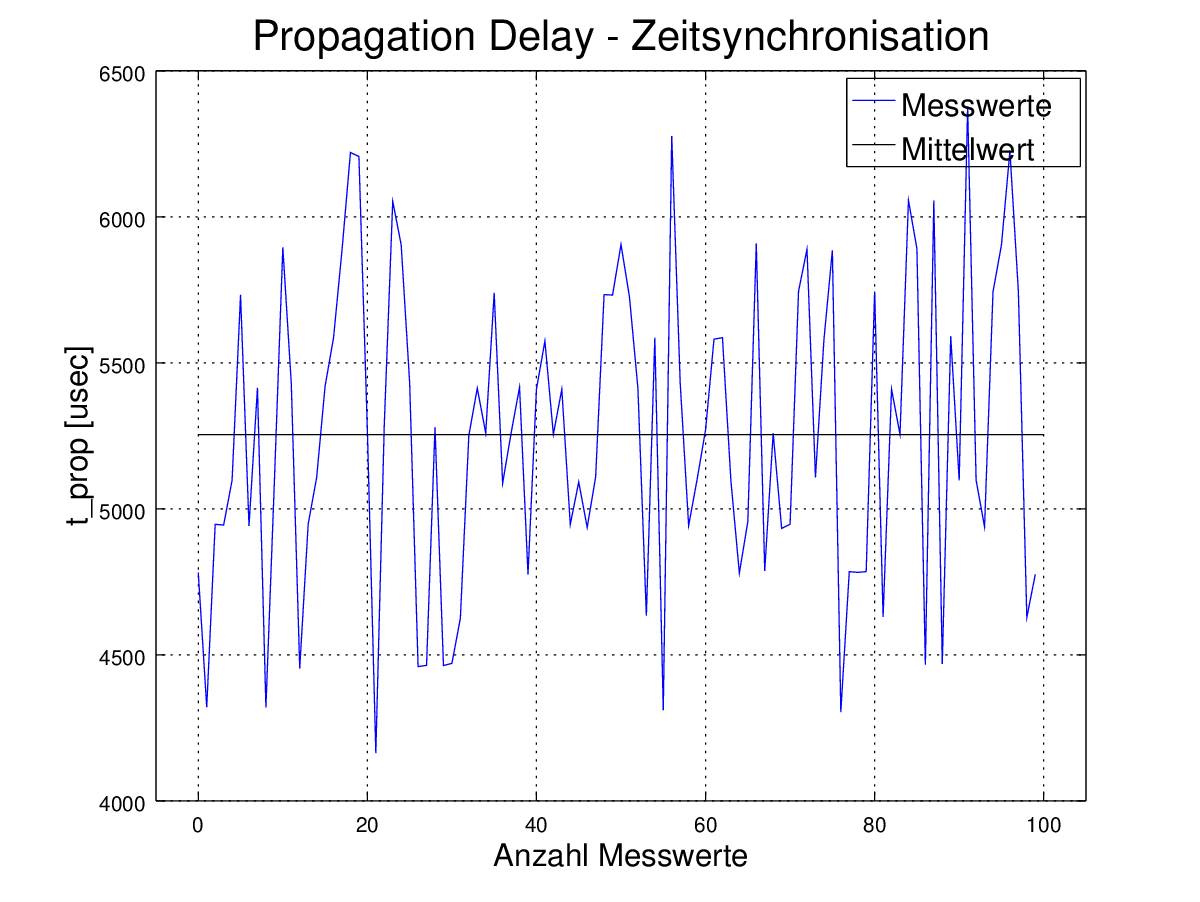
\includegraphics[width=1.2\textwidth]{images/t_prop_zeit_sync_figure.png}
\caption{Messwerte von $t_{prop}$ bei hundert Messungen}
\label{img:zeit_sync_t_prop_figure}
\end{figure}

\subsection{\funkempfaenger}
Um die Abweichung der Zeitsynchronisation aufzufangen, wird der \funkempfaenger \platz für das Startsignal einer Messung verwendet. Dafür muss allerdings der Empfänger ein eindeutiges Signal erhalten. Dies ist ein \si{LOW}-Signal. Da eine solche Abweichung für eine zentimetergenaue Positionsbestimmung nicht vertretbar ist, wird für den Start der Messung ein \funkempfaenger \platz verwendet. Für den Testaufbau wurde der Empfänger an das Oszilloskop angeschlossen. Der \si{DATA}-Eingang des Senders wurde mit dem \board \platz verbunden. Das Board produziert eine \SI{1}{\hertz} Frequenz auf dem verbundenen Pin. Das Oszilloskop sollte nun diese Frequenz widerspiegeln. Das Messergebnis ist in Abbildung \ref{img:ausgang_sender_pin} dargestellt. Das Mikrofon erkennt nur ein Rauschen. Dies bestätigen auch die vielen kurzen \si{LOW}-Pegel. Als vom Sender ein \si{LOW}-Pegel übertragen wurde, konnte nicht eindeutig bestimmt werden, ob das Signal angekommen war oder durch das Rauschen unterging. Die Pegelwechsel A-E belegen, dass sich kein Pegelwechsel am Ausgang eindeutig vom Rauschen abhebt. Somit kann diese Variante nicht als Startsignal verwendet werden. Der Funkempfänger scheidet damit aus.

\begin{figure}[H]
\centering
\hspace*{-1.7cm}
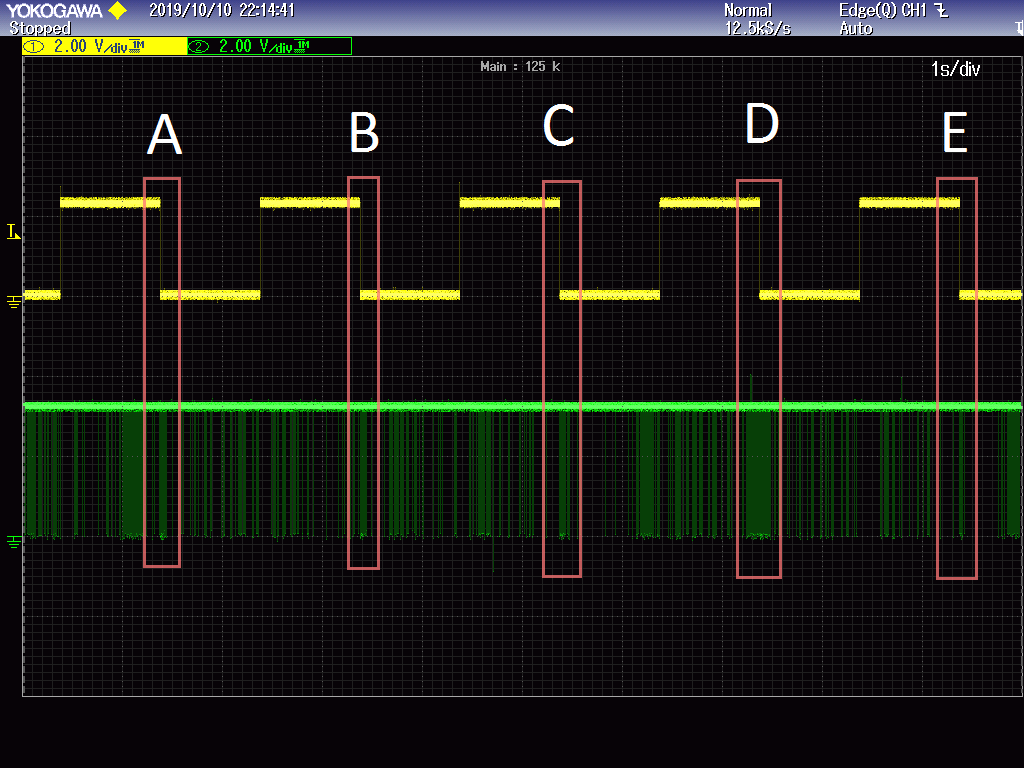
\includegraphics[width=1.2\textwidth]{images/schmitt_trigger_billig_sender_bearbeitet.png}
\caption{\si{DATA}-Pin des \funkempfaenger \platz Empfänger}
\label{img:ausgang_sender_pin}
\end{figure}

\subsection{Software}
Für die Positionsbestimmung verhält sich die Software nach dem Programmablaufplan (Abbildung \ref{img:PAP}). Zuerst wird der Zeitunterschied ausgeglichen, der zwischen dem Master und dem Slave besteht. Dafür wird das bereits beschriebene PTP Protokoll verwendet. Erst nachdem die Zeitsynchronisation erfolgreich ist, werden Messungen vorgenommen. Dabei spricht der Master einzeln die Slaves an. Der Master gibt zu einem bestimmten Zeitpunkt vor, wann der entsprechende Slave den Lautsprecher für \SI{40000}{\mu\s} einschaltet. Über das Mikrofon beim Master wird der Ton empfangen und sofort die Systemzeit bestimmt. Über die Differenz vom Aussenden und Empfangen kann die Distanz berechnet werden. Dieses Vorgehen wird für alle drei Slaves wiederholt. Zusammen mit den Koordinaten der Slaves ergeben sich auf einer Ebene drei Kreise, die sich schneiden. Der Schnittpunkt der Kreise ist folglich die Position des Masters. Dabei ist zu beachten, dass der Master sich während der drei Messungen nicht bewegen darf, sonst werden die Ergebnisse verfälscht. Mit den drei Distanzen wird die Position bestimmt. Die Funktion für die Positionsbestimmung wurde von Github (pepebecker/circle-intersection) entnommen \cite{src_GITHUB_CODE}. Wird die Software nicht abgebrochen, wiederholt sich die Messung für alle Slaves. Somit kann sich der Master auf der Ebene bewegen und bekommt seine Postion angezeigt. Es muss berücksichtigt werden, dass durch den Jitter des Frequenzgebers die Systemzeit der Slaves mit der Zeit divergiert, d.h, wartet man entsprechend lange, ist die Systemzeit der Slaves nicht mehr übereinstimmend mit dem Master. Deswegen muss regelmäßig eine Zeitsynchronisation erfolgen.

\begin{figure}[H]
\centering
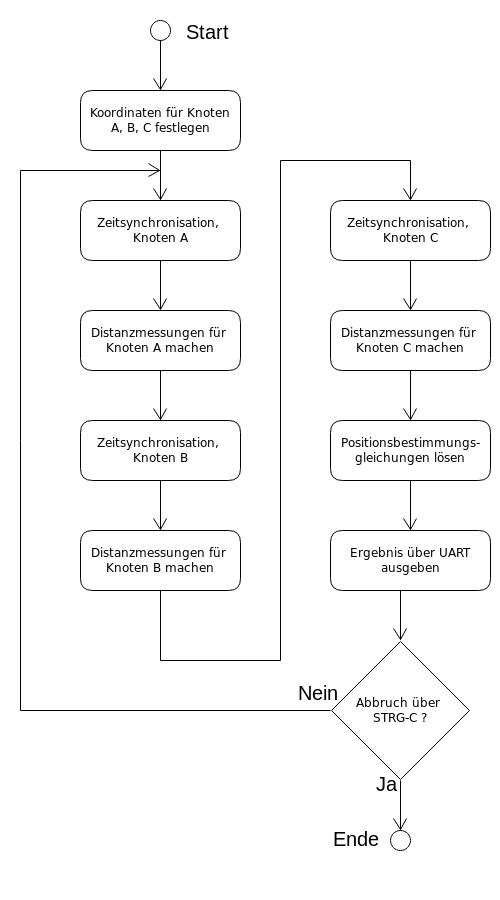
\includegraphics[width=0.8\textwidth]{images/PAP.png}
\caption{Programmablaufplan der Software}
\label{img:PAP}
\end{figure}




















